\documentclass{article}
\usepackage[T1]{fontenc}
\usepackage{lmodern}
\usepackage{graphicx}
\usepackage{amsmath,amssymb}
\usepackage[a4paper,margin=2cm]{geometry}
\usepackage[absolute,overlay]{textpos}
\setlength{\TPHorizModule}{1mm}
\setlength{\TPVertModule}{1mm}
\usepackage[indonesian]{babel}
\usepackage{hyperref}
\setlength{\emergencystretch}{2em}
\title{18-ECC-Bagian2-2026}
\author{pdf\_ppt\_to\_latex}
\date{}

\begin{document}

% --- unit llm 1 ---
% === Halaman 1 (llm) ===

\begin{center}
Bahan kuliah IF4020 Kriptografi

{\Huge Elliptic Curve Cryptography (ECC)}

\vspace{110.48mm}

{\Large (Bagian 2)}

\vspace{30mm}

Oleh: Rinaldi Munir

\vspace{10mm}

Program Studi Teknik Informatika\\
Sekolah Teknik Elektro dan Informatika\\
Institut Teknologi Bandung\\
2026
\end{center}

% deskripsi: Ilustrasi geometris penjumlahan titik pada kurva eliptik yang menunjukkan titik P, Q, hasil operasi P*Q, dan hasil refleksi P+Q
% bbox normalisasi: [0.7370, 0.3040, 0.9580, 0.6760]
\begin{textblock*}{46.41mm}(154.77mm,90.29mm)
\noindent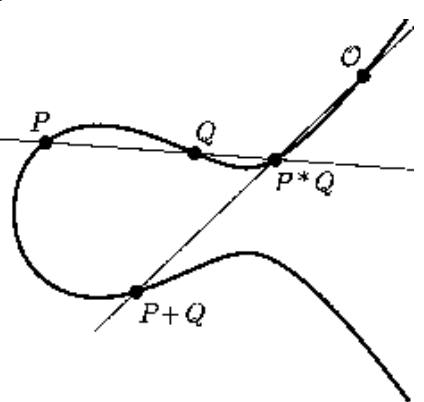
\includegraphics[width=46.41mm,height=110.48mm]{images/llm/page_001_img_01.png}%
\end{textblock*}

\newpage

% --- unit llm 2 ---
% === Halaman 2 (llm) ===

\section*{Pendahuluan}

\begin{itemize}
    \item Sebagian besar kriptografi kunci-publik (seperti RSA, ElGamal, Diffie-Hellman) menggunakan bilangan bulat yang sangat besar dalam komputasinya.
    \item Sistem seperti itu memiliki masalah yang signifikan dalam menyimpan, memproses kunci dan pesan, dan membutuhkan waktu komputasi yang lama.
    \item Sebagai alternatif adalah melakukan komputasi berbasis kurva eliptik (\textit{elliptic curve}).
    \item Kriptografi yang menggunakan kurva eliptik dinamakan \textit{Elliptic Curve Cryptography} (ECC).
    \item Komputasi dengan kurva eliptik menawarkan keamanan yang sama dengan algoritma-algoritma tersebut namun dengan ukuran kunci yang lebih kecil.
\end{itemize}

\vfill
\raggedleft{\small Sumber: William Stallings, Cryptography and Network Security\\
Chapter 10, 5$^{th}$ Edition}

\newpage

% --- unit llm 3 ---
% === Halaman 3 (llm) ===

\begin{itemize}
  \item ECC adalah kriptografi kunci-publik yang relatif lebih baru usianya.
  \item Dikembangkan oleh Neal Koblitz dan Victor S. Miller tahun 1985.
  \item Klaim: Panjang kunci ECC lebih pendek daripada kunci RSA, namun memiliki tingkat keamanan yang sama dengan RSA.
  \item Contoh: kunci ECC sepanjang 160-bit menyediakan tingkat keamanan yang sama dengan 1024-bit kunci RSA.
  \item Keuntungan: dengan panjang kunci yang lebih pendek, membutuhkan memori dan komputasi yang lebih sedikit.
  \item Cocok untuk piranti nirkabel, dimana prosesor, memori, umur batere terbatas.
\end{itemize}

\newpage

% --- unit llm 4 ---
% === Halaman 4 (llm) ===

\section*{Kurva Eliptik}

\begin{itemize}
    \item Kurva eliptik adalah kurva dengan bentuk umum persamaan:
    \[ y^2 = x^3 + ax + b \]
    dengan syarat $4a^3 + 27b^2 \neq 0$
    \item Tiap nilai a dan b yang berbeda memberikan kurva eliptik yang berbeda pula.
\end{itemize}

\newpage

% --- unit llm 5 ---
% === Halaman 5 (llm) ===

\begin{itemize}
  \item Contoh: \[ y^2 = x^3 - 4x \\ = x(x-2)(x+2) \]
\end{itemize}

\vspace{80mm}

\textcolor{red}{Sumber gambar: Andreas Steffen, Elliptic Curve Cryptography}

% deskripsi: Grafik kurva eliptik y^2 = x^3 - 4x yang terdiri dari sebuah loop tertutup dan sebuah kurva terbuka di sisi kanan.
% bbox normalisasi: [0.2150, 0.2540, 0.5870, 0.8240]
\begin{textblock*}{78.12mm}(45.15mm,75.44mm)
\noindent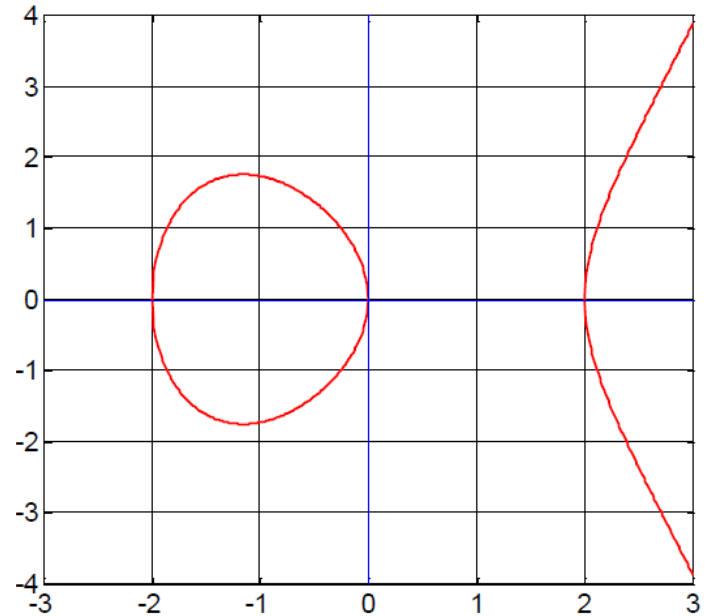
\includegraphics[width=78.12mm,height=169.29mm]{images/llm/page_005_img_01.png}%
\end{textblock*}

\newpage

% --- unit llm 6 ---
% === Halaman 6 (llm) ===

\vspace{209.98mm}

\begin{equation*}
  y^2 = x^3 - 12x + 13
\end{equation*}

\vspace{10mm}

Sumber gambar: Kevin Tirtawinata, Studi dan Analisis Elliptic Curve Cryptography

% deskripsi: Grafik kurva eliptik berdasarkan persamaan y^2 = x^3 - 12x + 13 pada bidang koordinat Kartesius.
% bbox normalisasi: [0.2850, 0.1130, 0.6600, 0.8200]
\begin{textblock*}{78.75mm}(59.85mm,33.56mm)
\noindent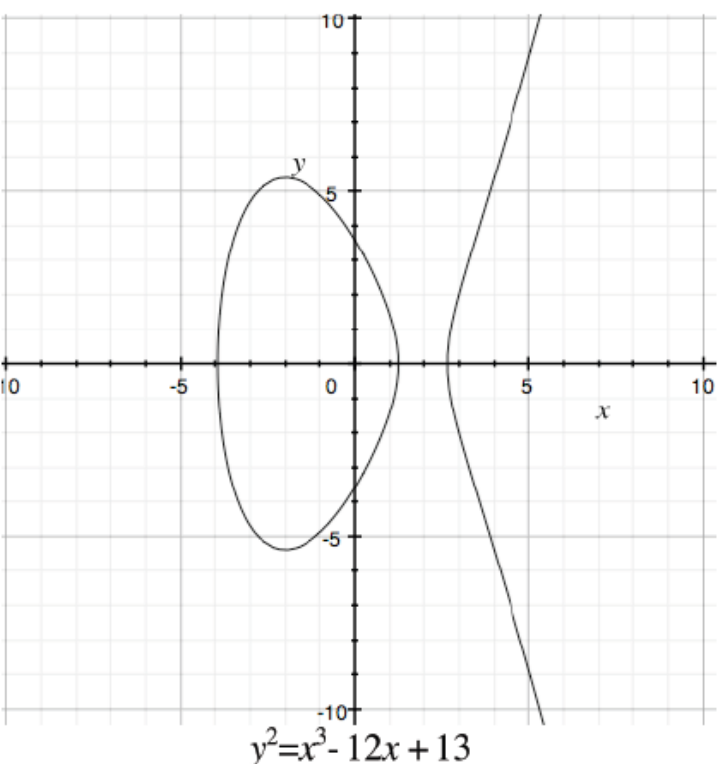
\includegraphics[width=78.75mm,height=209.98mm]{images/llm/page_006_img_01.png}%
\end{textblock*}

\newpage

% --- unit llm 7 ---
% === Halaman 7 (llm) ===

\vspace{80mm}

Sumber gambar: Kevin Tirtawinata, Studi dan Analisis Elliptic Curve Cryptography

% deskripsi: Grafik kurva eliptik dengan persamaan y^2 = x^3 - 10x + 13 pada koordinat Kartesius.
% bbox normalisasi: [0.3600, 0.3400, 0.6350, 0.8200]
\begin{textblock*}{57.75mm}(75.60mm,100.98mm)
\noindent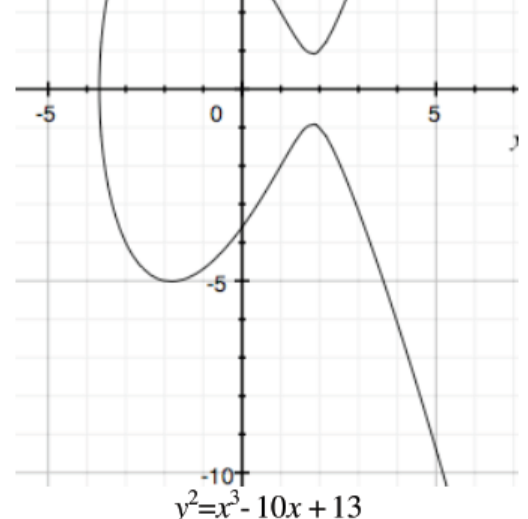
\includegraphics[width=57.75mm,height=142.56mm]{images/llm/page_007_img_01.png}%
\end{textblock*}

\newpage

% --- unit llm 8 ---
% === Halaman 8 (llm) ===

\vspace{30mm}

Sumber gambar: \textbf{Debdeep Mukhopadhyay, Elliptic Curve Cryptography}, \\
Dept of Computer Sc and Engg IIT Madras

% deskripsi: Kumpulan lima grafik kurva eliptik dengan persamaan yang berbeda: y^2 = x^3 - 1, y^2 = x^3 + 1, y^2 = x^3 - 3x + 3, y^2 = x^3 - 4x, dan y^2 = x^3 - x.
% bbox normalisasi: [0.1800, 0.3000, 0.8300, 0.5600]
\begin{textblock*}{136.50mm}(37.80mm,89.10mm)
\noindent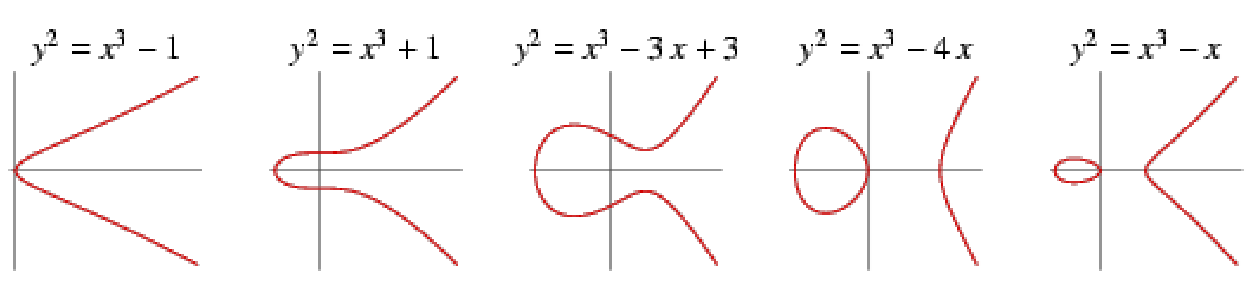
\includegraphics[width=136.50mm,height=77.22mm]{images/llm/page_008_img_01.png}%
\end{textblock*}

\newpage

% --- unit llm 9 ---
% === Halaman 9 (llm) ===

\begin{itemize}
    \item Kurva eliptik $y^2 = x^3 + ax + b$ terdefinisi untuk $x, y \in \mathbb{R}$
    \item Didefinisikan sebuah titik bernama titik $O(x, \infty)$, yaitu titik pada \textit{infinity}.
    \item Titik-titik $P(x, y)$ pada kurva eliptik bersama operasi $+$ membentuk sebuah grup.
    \begin{itemize}
        \item Himpunan $G$ : semua titik $P(x, y)$ pada kurva eliptik
        \item Operasi biner : $+$
    \end{itemize}
    \item Penjelasan kenapa kurva eliptik membentuk sebuah grup dijelaskan pada \textit{slide-slide} berikut ini.
\end{itemize}

\newpage

% --- unit llm 10 ---
% === Halaman 10 (llm) ===

\section*{Penjumlahan Titik pada Kurva Eliptik}

\vspace{190.08mm}

(a) $P + Q = R$

Penjelasan geometri:
\begin{enumerate}
  \item Tarik garis melalui $P$ dan $Q$
  \item Jika $P \neq Q$, garis tersebut memotong kurva pada titik $-R$
  \item Pencerminan titik $-R$ terhadap sumbu-x adalah titik $R$
  \item Titik $R$ adalah hasil penjumlahan titik $P$ dan $Q$
\end{enumerate}

\vspace{10mm}

Keterangan: Jika $R=(x, y)$ maka $-R$ adalah titik $(x, -y)$

\vspace{5mm}

\centering Sumber gambar: Andreas Steffen, Elliptic Curve Cryptography

% deskripsi: Grafik kurva eliptik yang mengilustrasikan geometri penjumlahan dua titik P dan Q untuk mendapatkan titik R, termasuk garis bantu dan titik -R sebagai hasil refleksi terhadap sumbu-x.
% bbox normalisasi: [0.4500, 0.2000, 0.8700, 0.8400]
\begin{textblock*}{88.20mm}(94.50mm,59.40mm)
\noindent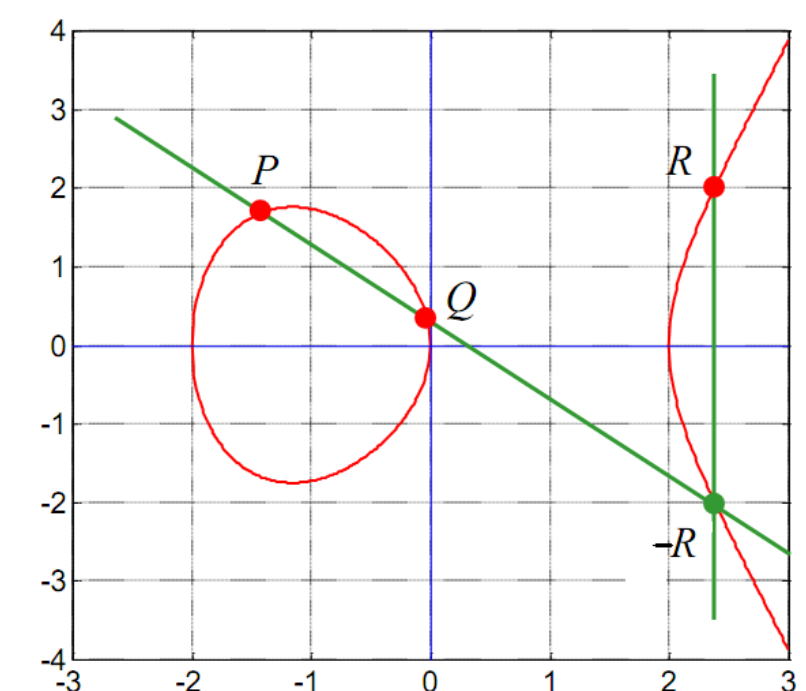
\includegraphics[width=88.20mm,height=190.08mm]{images/llm/page_010_img_01.png}%
\end{textblock*}

\newpage

% --- unit llm 11 ---
% === Halaman 11 (llm) ===

\section*{Penjelasan Analitik P + Q = R}

Persamaan garis g: \[ y = mx + c \]

\vspace{160.38mm}

Gradien garis g: \[ m = \frac{y_p - y_q}{x_p - x_q} \]

Perpotongan garis g dengan kurva $y^2 = x^3 + ax + b$ adalah:
\[ (mx + c)^2 = x^3 + ax + b \]

\vspace{50mm}

Koordinat Titik R:
\[
\begin{aligned}
x_r &= m^2 - x_p - x_q \\
y_r &= m(x_p - x_r) - y_p
\end{aligned}
\]

\vspace{10mm}
\hfill \textcolor{red}{Sumber gambar: Andreas Steffen, Elliptic Curve Cryptography}

% deskripsi: Grafik kurva eliptik dengan garis g yang memotong titik P, Q, dan -R, serta proyeksi titik -R ke titik R
% bbox normalisasi: [0.5150, 0.2300, 0.8650, 0.7700]
\begin{textblock*}{73.50mm}(108.15mm,68.31mm)
\noindent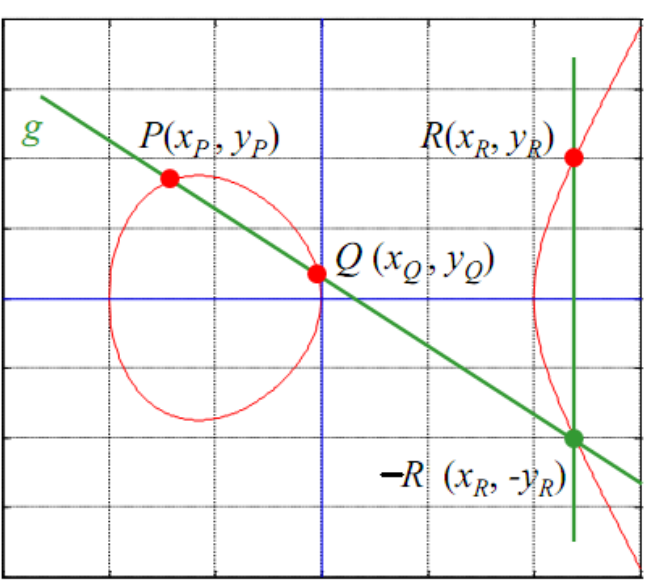
\includegraphics[width=73.50mm,height=160.38mm]{images/llm/page_011_img_01.png}%
\end{textblock*}

\newpage

% --- unit llm 12 ---
% === Halaman 12 (llm) ===

Contoh: Kurva eliptik $y^2 = x^3 + 2x + 4$

Misalkan $P(2, 4)$ dan $Q(0, 2)$ dua titik pada kurva

Penjumlahan titik: $P + Q = R$. Tentukan $R$!

Langkah-langkah menghitung koordinat $R$:

\begin{itemize}
    \item Gradien garis $g$: $m = (y_p - y_q)/(x_p - x_q) = (4 - 2)/(2 - 0) = 1$
    \item $x_r = m^2 - x_p - x_q = 1^2 - 2 - 0 = -1$
    \item $y_r = m(x_p - x_r) - y_p = 1(2 - (-1)) - 4 = -1$
    \item Jadi koordinat $R(-1, -1)$
    \item Periksa apakah $R(-1, -1)$ sebuah titik pada kurva eliptik:
    
    \begin{align*}
    y^2 = x^3 + 2x + 4 & \Leftrightarrow (-1)^2 = (-1)^3 + 2(-1) + 4 \\
    & \Leftrightarrow 1 = -1 - 2 + 4 \\
    & \Leftrightarrow 1 = 1 \text{ (terbukti } R(-1, -1) \text{ titik yang terletak pada kurva } y^2 = x^3 + 2x + 4)\
    \end{align*}
\end{itemize}

\newpage

% --- unit llm 13 ---
% === Halaman 13 (llm) ===

\bullet Contoh lain:

\vspace{197.21mm}

\begin{align*}
 m &= (y_p - y_q)/(x_p - x_q) \\
 &= (-1.86 - 0.836)/(-2.35 - (-0.1)) \\
 &= -2.696 / -2.25 = 1.198 
\end{align*}

\begin{align*}
 x_r &= m^2 - x_p - x_q \\
 &= (1.198)^2 - (-2.35) - (-0.1) \\
 &= 3.89 
\end{align*}

\begin{align*}
 y_r &= m(x_p - x_r) - y_p \\
 &= 1.198(-2.35 - 3.89) - (-1.86) \\
 &= -5.62 
\end{align*}

\vspace{10mm}

Sumber gambar: Debdeep Mukhopadhyay, Elliptic Curve Cryptography, Dept of Computer Sc Engg IIT Madras

% deskripsi: Grafik kurva eliptik $y^2 = x^3 - 7x$ yang menunjukkan operasi penjumlahan titik $P + Q = R$, lengkap dengan garis bantu dan koordinat titik P, Q, R, dan -R.
% bbox normalisasi: [0.5050, 0.1260, 0.9200, 0.7900]
\begin{textblock*}{87.15mm}(106.05mm,37.42mm)
\noindent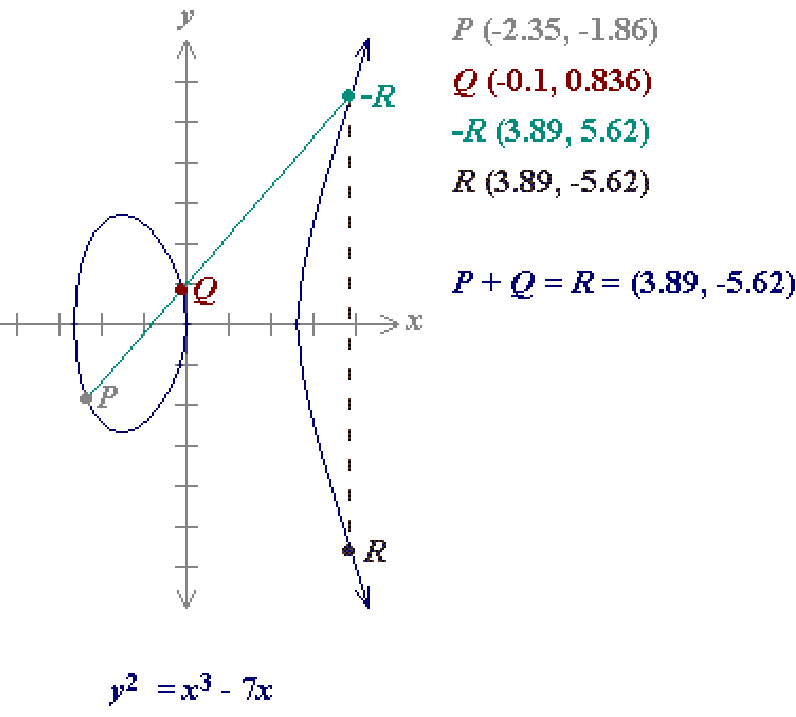
\includegraphics[width=87.15mm,height=197.21mm]{images/llm/page_013_img_01.png}%
\end{textblock*}

\newpage

% --- unit llm 14 ---
% === Halaman 14 (llm) ===

\vspace{237.60mm}

Demo kalkulkator ECC online: \url{https://andrea.corbellini.name/ecc/interactive/reals-add.html}

\vspace{10mm}

Point addition over the elliptic curve \[ y^2 = x^3 - 7x + 10 \] in $\mathbb{R}$.

% deskripsi: Tangkapan layar kalkulator interaktif Elliptic Curve point addition yang menunjukkan grafik kurva eliptik, garis yang menghubungkan titik P dan Q, serta input parameter kurva dan koordinat titik-titiknya.
% bbox normalisasi: [0.0400, 0.1600, 0.9500, 0.9600]
\begin{textblock*}{191.10mm}(8.40mm,47.52mm)
\noindent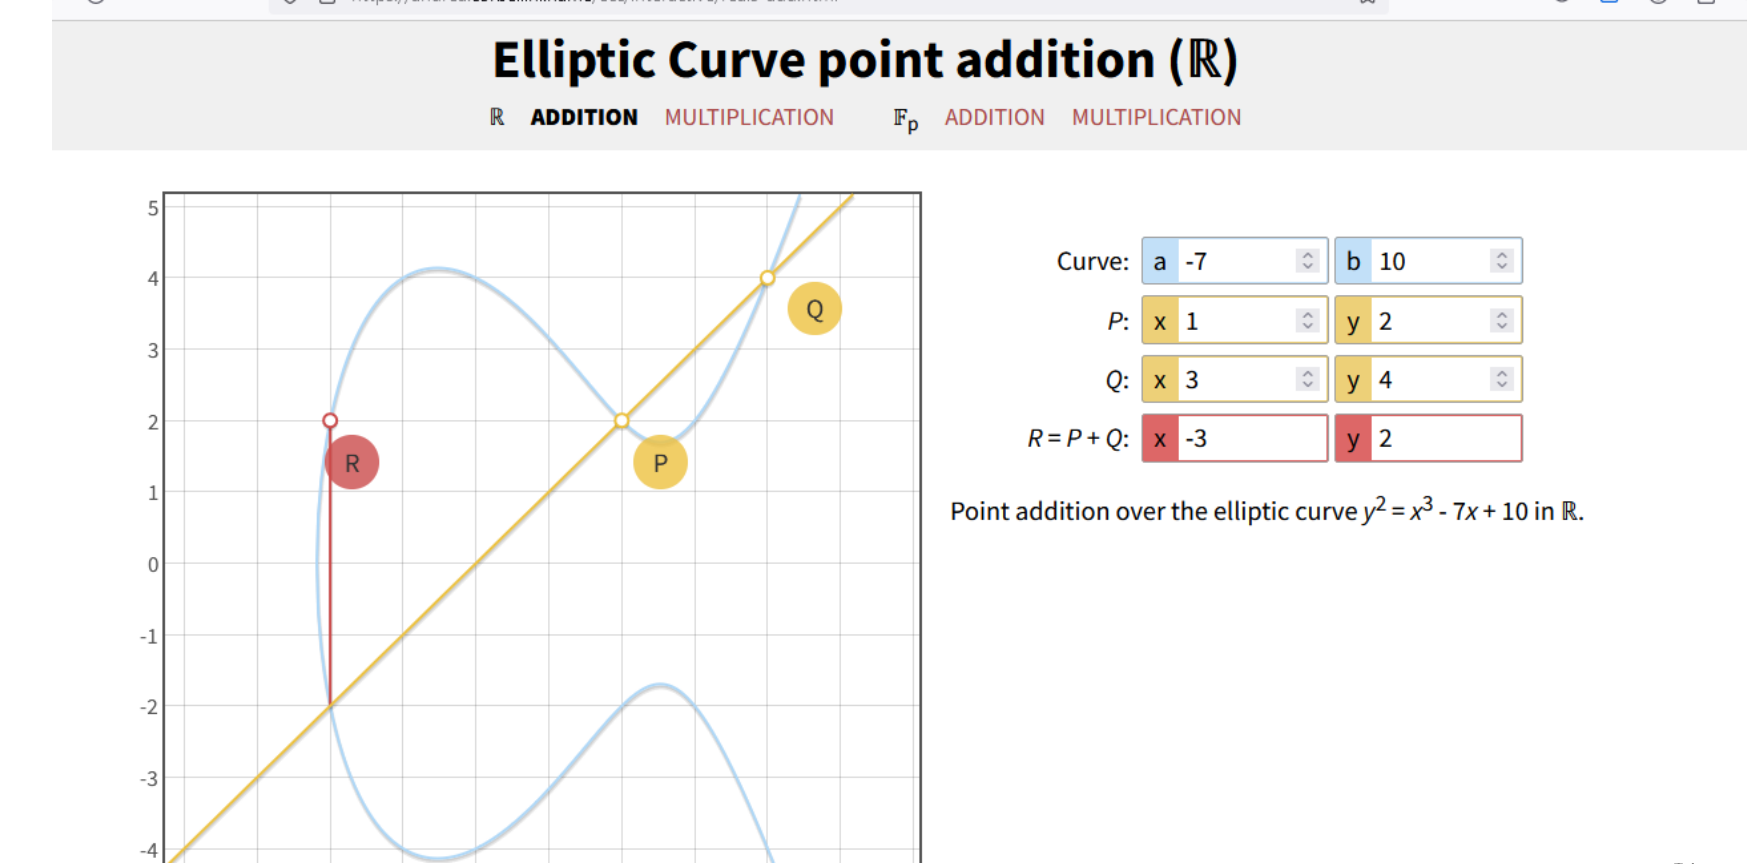
\includegraphics[width=191.10mm,height=237.60mm]{images/llm/page_014_img_01.png}%
\end{textblock*}

\newpage

% --- unit llm 15 ---
% === Halaman 15 (llm) ===

(b) $P + (-P) = O$, di sini $O$ adalah titik di $infinity$

\vspace{10mm}

$P' = -P$ adalah elemen invers:
\[ P + P' = P + (-P) = O \]

$O$ adalah elemen netral:
\[ P + O = O + P = P \]

\vspace{20mm}

\centering{\textcolor{red}{Sumber gambar: Andreas Steffen, Elliptic Curve Cryptography}}

% deskripsi: Grafik kurva eliptik pada koordinat Kartesius yang menunjukkan titik P dan inversnya -P, dengan garis bantu vertikal berwarna hijau yang melewati kedua titik tersebut.
% bbox normalisasi: [0.4740, 0.2030, 0.8440, 0.8170]
\begin{textblock*}{77.70mm}(99.54mm,60.29mm)
\noindent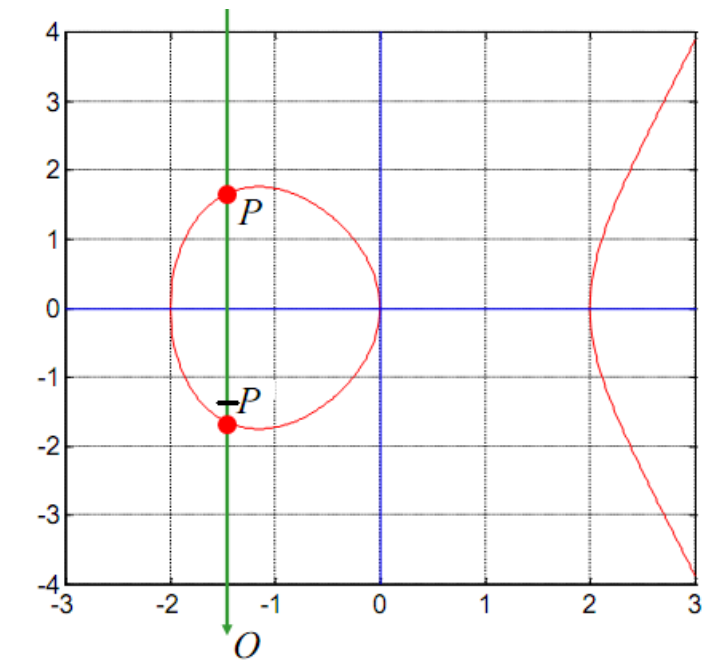
\includegraphics[width=77.70mm,height=182.36mm]{images/llm/page_015_img_01.png}%
\end{textblock*}

\newpage

% --- unit llm 16 ---
% === Halaman 16 (llm) ===

\section*{Penggandaan Titik}

\vspace{181.17mm}

\begin{itemize}
    \item Penggandaan titik (\textit{point doubling}): menjumlahkan sebuah titik pada dirinya sendiri
    \vspace{10mm}
    \item Penggandaan titik membentuk tangen pada titik $P(x, y)$
    \item $P + P = 2P = R$
\end{itemize}

\vspace{5mm}
\textcolor{red}{Sumber gambar: Andreas Steffen, Elliptic Curve Cryptography}

% deskripsi: Grafik kurva eliptik yang mengilustrasikan operasi penggandaan titik (point doubling), menunjukkan garis tangen di titik P, titik potong R, dan refleksinya -R.
% bbox normalisasi: [0.4500, 0.2300, 0.8800, 0.8400]
\begin{textblock*}{90.30mm}(94.50mm,68.31mm)
\noindent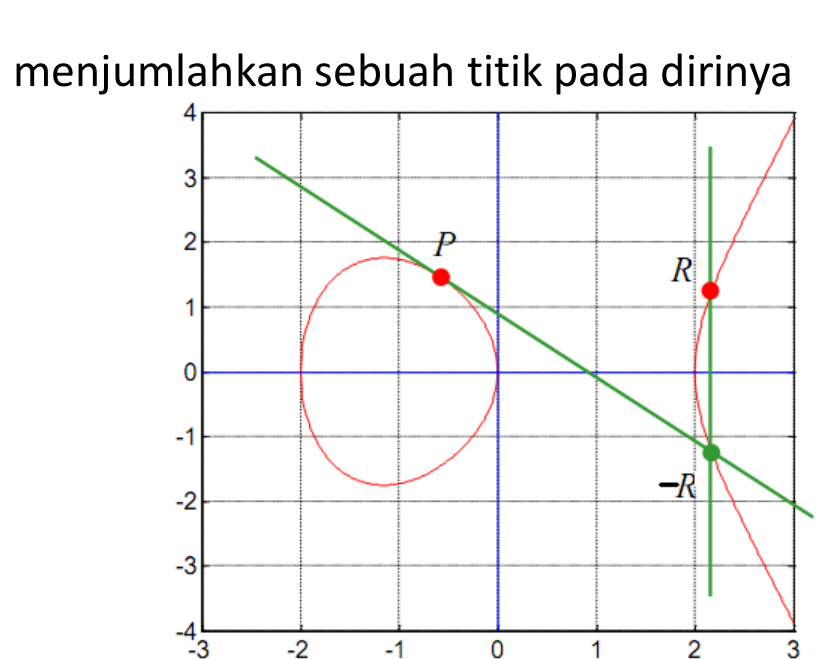
\includegraphics[width=90.30mm,height=181.17mm]{images/llm/page_016_img_01.png}%
\end{textblock*}

\newpage

% --- unit llm 17 ---
% === Halaman 17 (llm) ===

\begin{itemize}
    \item Jika ordinat titik P nol, yaitu $y_p = \text{nol}$, maka tangen pada titik tersebut berpotongan pada sebuah titik di \textit{infinity}.
    \vspace{10mm}
    \item Di sini, $P + P = 2P = O$
\end{itemize}

\vspace{10mm}

\textcolor{red}{\text{Sumber gambar: Anoop MS, Elliptic Curve Cryptography, an Implementation Guide}}

% deskripsi: Grafik kurva eliptik yang menunjukkan titik P pada sumbu x dengan garis singgung vertikal yang menuju ke titik tak hingga (infinity), lengkap dengan keterangan teks y_p = 0 hence 2P = O.
% bbox normalisasi: [0.5130, 0.2740, 0.8010, 0.8940]
\begin{textblock*}{60.48mm}(107.73mm,81.38mm)
\noindent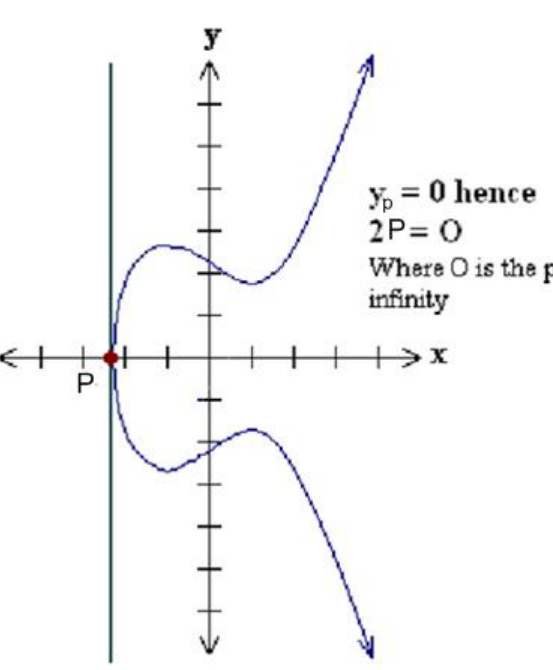
\includegraphics[width=60.48mm,height=184.14mm]{images/llm/page_017_img_01.png}%
\end{textblock*}

\newpage

% --- unit llm 18 ---
% === Halaman 18 (llm) ===

\section*{Penjelasan Analitik $P + P = 2P = R$}

Persamaan tangen $g$: $y = mx + c$

\vspace{157.41mm}

Gradien garis $g$: \[ m = \frac{dy}{dx} = \frac{3x_p^2 + a}{2y_p} \]

Perpotongan garis $g$ dengan kurva: $(mx + c)^2 = x^3 + ax + b$

Koordinat Titik R:
\begin{align*}
x_r &= m^2 - 2x_p \\
y_r &= m(x_p - x_r) - y_p
\end{align*}

Jika $y_p = 0$ maka $m$ tidak terdefinisi sehingga $2P = O$

\vspace{10mm}

Sumber gambar: Andreas Steffen, Elliptic Curve Cryptography

% deskripsi: Grafik kurva eliptik yang menunjukkan titik P, titik R, dan garis singgung g yang memotong kurva di titik P dan R, serta proyeksi titik -R
% bbox normalisasi: [0.5200, 0.2200, 0.8500, 0.7500]
\begin{textblock*}{69.30mm}(109.20mm,65.34mm)
\noindent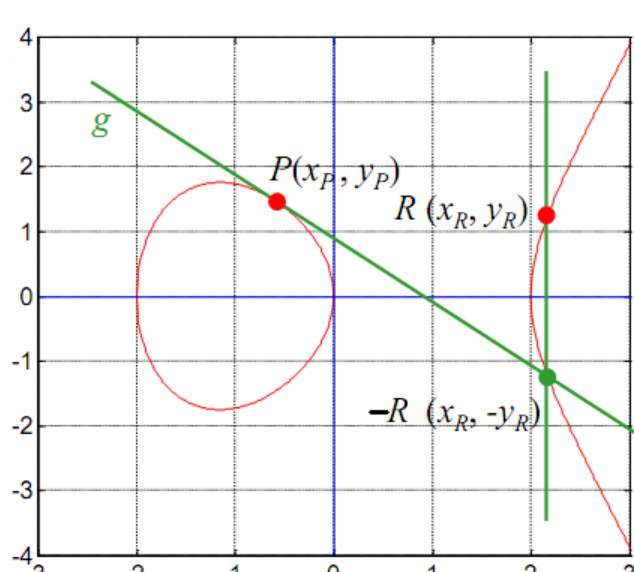
\includegraphics[width=69.30mm,height=157.41mm]{images/llm/page_018_img_01.png}%
\end{textblock*}

\newpage

% --- unit llm 19 ---
% === Halaman 19 (llm) ===

\begin{itemize}
    \item Contoh:
\end{itemize}

\[ P+P = 2P \]

\vspace{10mm}

\[ m = \frac{dy}{dx} = \frac{3x_p^2 + a}{2y_p} \]

Koordinat Titik R:
\[ x_r = m^2 - 2x_p \]
\[ y_r = m(x_p - x_r) - y_p \]

\vspace{40mm}

Sumber gambar: Debdeep Mukhopadhyay, Elliptic Curve Cryptography, Dept of Computer Sc and Engg IIT Madras

% deskripsi: Grafik kurva eliptik dengan persamaan y^2 = x^3 - 3x + 5 yang menunjukkan operasi penjumlahan titik P + P = 2P, lengkap dengan titik P, R, dan -R serta garis singgung.
% bbox normalisasi: [0.3900, 0.2200, 0.6700, 0.8200]
\begin{textblock*}{58.80mm}(81.90mm,65.34mm)
\noindent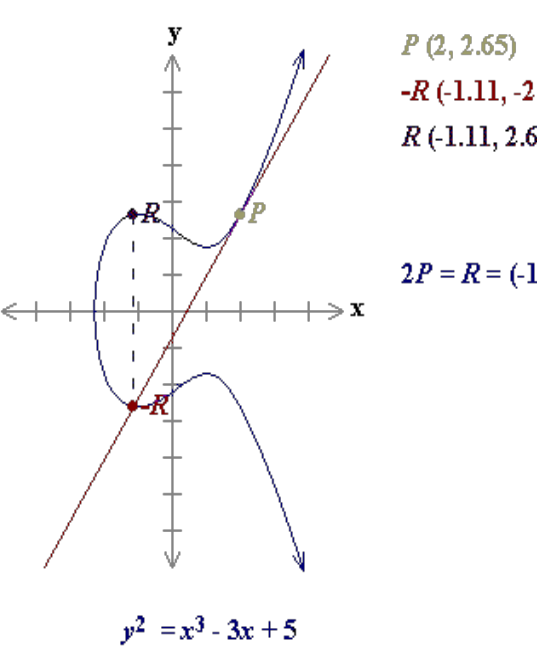
\includegraphics[width=58.80mm,height=178.20mm]{images/llm/page_019_img_01.png}%
\end{textblock*}

\newpage

% --- unit llm 20 ---
% === Halaman 20 (llm) ===

\section*{Pelelaran Titik}

\vspace{160.38mm}

\begin{itemize}
    \item Pelelaran titik (\textit{point iteration}): menjumlahkan sebuah titik sebanyak $k - 1$ kali terhadap dirinya sendiri.
    \item $P^k = kP = P + P + \dots + P$
    \item Jika $k = 2 \rightarrow P^2 = 2P = P + P$
\end{itemize}

\vspace{20mm}

\textcolor{red}{\text{Sumber gambar: Andreas Steffen, Elliptic Curve Cryptography}}

% deskripsi: Grafik ilustrasi operasi pelelaran titik pada kurva eliptik yang menunjukkan titik P, P^2, dan P^3 serta garis bantu yang digunakan dalam proses penjumlahan titik.
% bbox normalisasi: [0.5100, 0.3700, 0.8400, 0.9100]
\begin{textblock*}{69.30mm}(107.10mm,109.89mm)
\noindent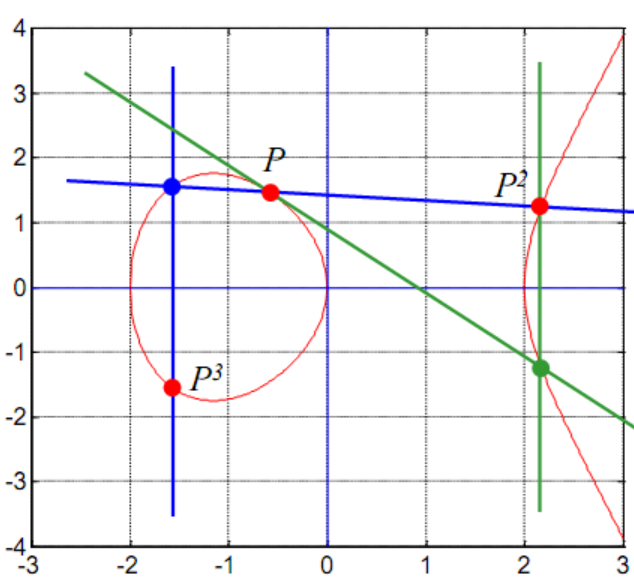
\includegraphics[width=69.30mm,height=160.38mm]{images/llm/page_020_img_01.png}%
\end{textblock*}

\newpage

% --- unit llm 21 ---
% === Halaman 21 (llm) ===

\section*{Jelaslah Kurva Eliptik membentuk Grup $\langle G, + \rangle$}

Karena:
\begin{itemize}
    \item Himpunan $G$: semua titik $P(x,y)$ pada kurva eliptik
    \item Operasi biner: $+$
    \item Semua aksioma terpenuhi sbb:
    \begin{enumerate}
        \item Closure: semua operasi $P + Q$ berada di dalam $G$
        \item Asosiatif: $P + (Q + R) = (P + Q) + R$
        \item Elemen netral adalah $O$: $P + O = O + P = P$
        \item Elemen invers adalah $-P$: $P + (-P) = O$
        \item Komutatif: $P + Q = Q + P$ \textcolor{red}{(abelian)}
    \end{enumerate}
\end{itemize}

\newpage

% --- unit llm 22 ---
% === Halaman 22 (llm) ===

\section*{Perkalian Titik}

\begin{itemize}
    \item Perkalian titik: \(kP = Q\)
    
    Ket: \(k\) adalah skalar, \(P\) dan \(Q\) adalah titik pada kurva eliptik
    
    \item Perkalian titik diperoleh dengan perulangan dua operasi dasar kurva eliptik yang sudah dijelaskan:
    \begin{enumerate}
        \item Penjumlahan titik \((P + Q = R)\)
        \item Penggandaan titik \((2P = R)\)
    \end{enumerate}
    
    \item Contoh: \(k = 3 \rightarrow 3P = P + P + P\) atau \(3P = 2P + P\)
    
    \(k = 23 \rightarrow kP = 23P = 2(2(2(2P) + P) + P) + P\)
\end{itemize}

\newpage

% --- unit llm 23 ---
% === Halaman 23 (llm) ===

\section*{Elliptic Curve Discrete Logarithm Problem (ECDLP)}

\begin{itemize}
    \item Menghitung $kP = Q$ mudah, tetapi menghitung $k$ jika diketahui $P$ dan $Q$ adalah sulit. Inilah ECDLP yang menjadi dasar ECC.
    \item ECDLP dirumuskan sebagai berikut:
    
    \textcolor{red}{Diberikan $P$ dan $Q$ adalah dua buah titik di kurva eliptik, carilah integer $k$ sedemikian sehingga $Q = kP$}
    
    \item Secara komputasi sulit menemukan $k$, jika $k$ adalah bilangan yang besar. Nilai $k$ adalah logaritma diskrit dari $Q$ dengan basis $P$. \textcolor{red}{*)}
    \item Pada algoritma ECC, $Q$ adalah kunci publik, $k$ adalah kunci privat, dan $P$ sembarang titik pada kurva eliptik.
\end{itemize}

\centering
\textcolor{red}{Catatan: ingatlah $kP = P^k$, sehingga $Q = kP = P^k$, $k$ adalah logaritma diskrit dari $Q$}

\newpage

% --- unit llm 24 ---
% === Halaman 24 (llm) ===

\section*{Kurva Eliptik pada Galois Field}

\begin{itemize}
    \item Operasi kurva eliptik yang dibahas sebelum ini didefinisikan pada bilangan riil.
    \item Operasi pada bilangan riil tidak akurat karena mengandung pembulatan
    \item Pada sisi lain, kriptografi dioperasikan pada ranah bilangan integer.
    \item Agar kurva eliptik dapat dipakai di dalam kriptografi, maka kurva eliptik didefinisikan pada medan berhingga atau Galois Field, yaitu $\text{GF}(p)$ dan $\text{GF}(2^m)$.
    \item Yang dibahas dalam kuliah ini hanya kurva eliptik pada $\text{GF}(p)$
\end{itemize}

\newpage

% --- unit llm 25 ---
% === Halaman 25 (llm) ===

\section*{Kurva Eliptik pada GF(p)}

\begin{itemize}
    \item Bentuk umum kurva eliptik pada GF(p) (atau $\text{F}_p$) :
\end{itemize}

\[ y^2 \equiv x^3 + ax + b \pmod{p} \]

\vspace{10mm}

yang dalam hal ini $p$ adalah bilangan prima dan elemen-elemen himpunan di dalam medan galois adalah $\{0, 1, 2, \dots, p-1\}$

\newpage

% --- unit llm 26 ---
% === Halaman 26 (llm) ===

\begin{itemize}
    \item \textbf{Contoh:} Tentukan semua titik $\text{P}(\text{x},\text{y})$ pada kurva eliptik
    \[ y^2 \equiv x^3 + x + 6 \pmod{11} \]
    dengan $\text{x}$ dan $\text{y}$ didefinisikan di dalam $\text{GF}(11)$
\end{itemize}

\textbf{Jawab:}

\begin{align*}
    \text{x} = 0 & \rightarrow y^2 \equiv 6 \pmod{11} \rightarrow \text{tidak ada nilai y yang memenuhi} \\
    \text{x} = 1 & \rightarrow y^2 \equiv 8 \pmod{11} \rightarrow \text{tidak ada nilai y yang memenuhi} \\
    \text{x} = 2 & \rightarrow y^2 \equiv 16 \pmod{11} \equiv 5 \pmod{11} \rightarrow y_1 = 4 \text{ dan } y_2 = 7 \\
    & \rightarrow \text{titik } \text{P}(2,4) \text{ dan } \text{P}'(2,7) \\
    \text{x} = 3 & \rightarrow y^2 \equiv 36 \pmod{11} \equiv 3 \pmod{11} \rightarrow y_1 = 5 \text{ dan } y_2 = 6 \\
    & \rightarrow \text{titik } \text{P}(3,5) \text{ dan } \text{P}'(3,6)
\end{align*}

\newpage

% --- unit llm 27 ---
% === Halaman 27 (llm) ===

Jika diteruskan untuk $x = 4, 5, \dots, 10$, diperoleh tabel sebagai berikut :

\vspace{10mm}

Jadi, titik-titik yang terdapat pada kurva eliptik adalah 12, yaitu:
(2, 4), (2, 7), (3, 5), (3, 6), (5, 2), (5, 9), (7, 2), (7, 9), (8, 3), (8, 8), (10, 2), (10, 9)

\vspace{5mm}

Jika ditambah dengan titik O di infinity, maka titik-titik pada kurva eliptik membentuk grup dengan $n = 13$ elemen.

\vspace{10mm}

\begin{flushright}
\textcolor{red}{Sumber: Andreas Steffen, \\
Elliptic Curve Cryptography}
\end{flushright}

% deskripsi: Tabel perhitungan nilai x, y^2, y_{1,2}, P(x,y), dan P'(x,y) untuk kurva eliptik dengan beberapa coretan tangan penanda.
% bbox normalisasi: [0.1800, 0.2200, 0.4700, 0.8300]
\begin{textblock*}{60.90mm}(37.80mm,65.34mm)
\noindent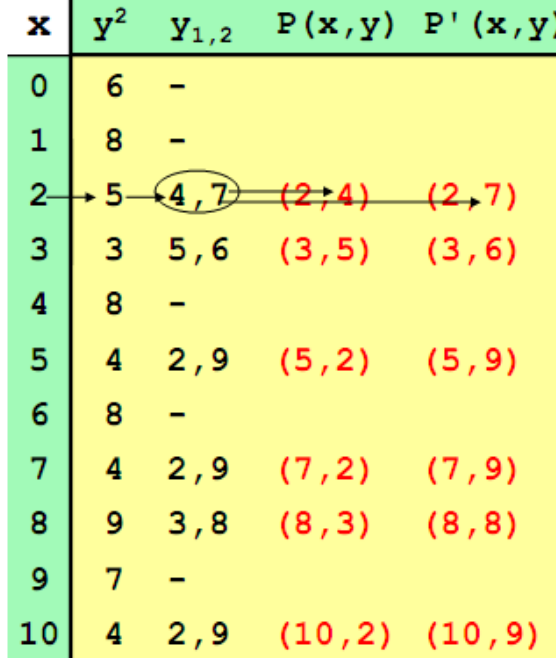
\includegraphics[width=60.90mm,height=181.17mm]{images/llm/page_027_img_01.png}%
\end{textblock*}

\newpage

% --- unit llm 28 ---
% === Halaman 28 (llm) ===

\vspace{193.05mm}

\vspace{60mm}
Sebaran titik di dalam kurva eliptik $y^2 = x^3 + x + 6 \pmod{11}$ pada $\text{GF}(11)$

% deskripsi: Grafik sebaran titik (scatter plot) dari persamaan kurva eliptik $y^2 = x^3 + x + 6 \pmod{11}$ pada bidang koordinat dengan sumbu x dari 0 sampai 10 dan sumbu y dari 0 sampai 10.
% bbox normalisasi: [0.2000, 0.1000, 0.7500, 0.7500]
\begin{textblock*}{115.50mm}(42.00mm,29.70mm)
\noindent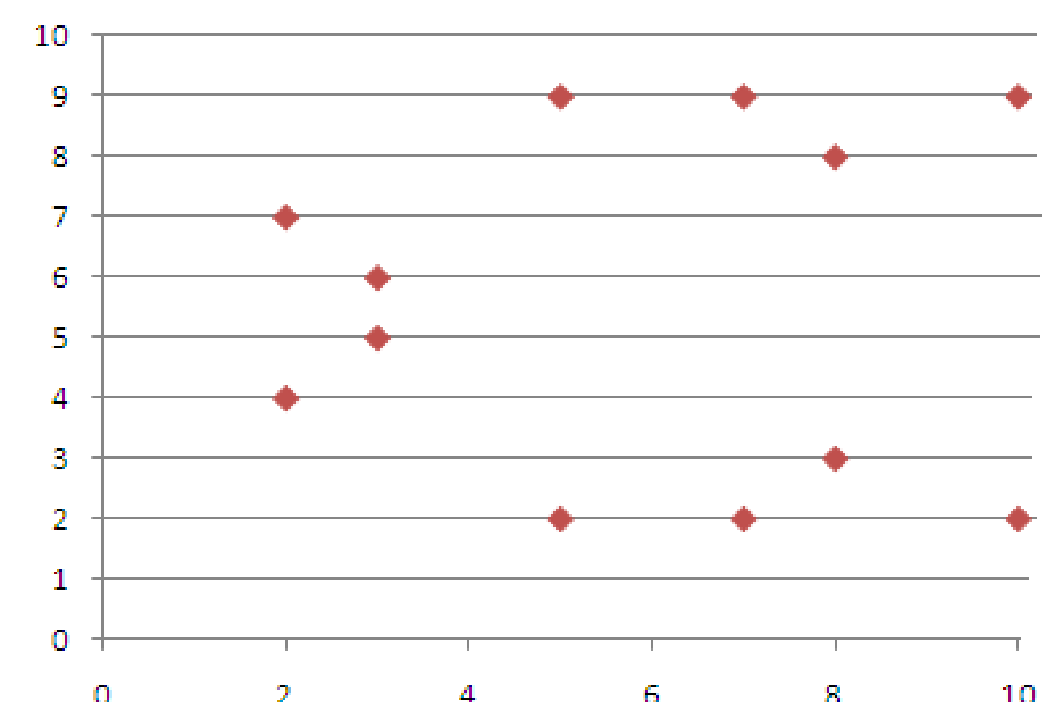
\includegraphics[width=115.50mm,height=193.05mm]{images/llm/page_028_img_01.png}%
\end{textblock*}

\newpage

% --- unit llm 29 ---
% === Halaman 29 (llm) ===

\begin{itemize}
    \item Contoh lain: Kurva eliptik $y^2 \equiv x^3 + x + 1 \pmod{23}$ memiliki titik-titik di dalam himpunan $\{(0, 1), (0, 22), (1, 7), (1, 16), (3, 10), (3, 13), (5, 4), (5, 19), (6, 4), (6, 19), (7, 11), (7, 12), (9, 7), (9, 16), (11, 3), (11, 20), (12, 4), (12, 19), (13, 7), (13, 16), (17, 3), (17, 20), (18, 3), (18, 20), (19, 5), (19, 18)\}$.
\end{itemize}

\vspace{10mm}

% deskripsi: Grafik scatter plot yang menunjukkan titik-titik solusi dari persamaan kurva eliptik $y^2 \equiv x^3 + x + 1 \pmod{23}$ pada bidang koordinat x dan y.
% bbox normalisasi: [0.2040, 0.3210, 0.7680, 0.8560]
\begin{textblock*}{118.44mm}(42.84mm,95.34mm)
\noindent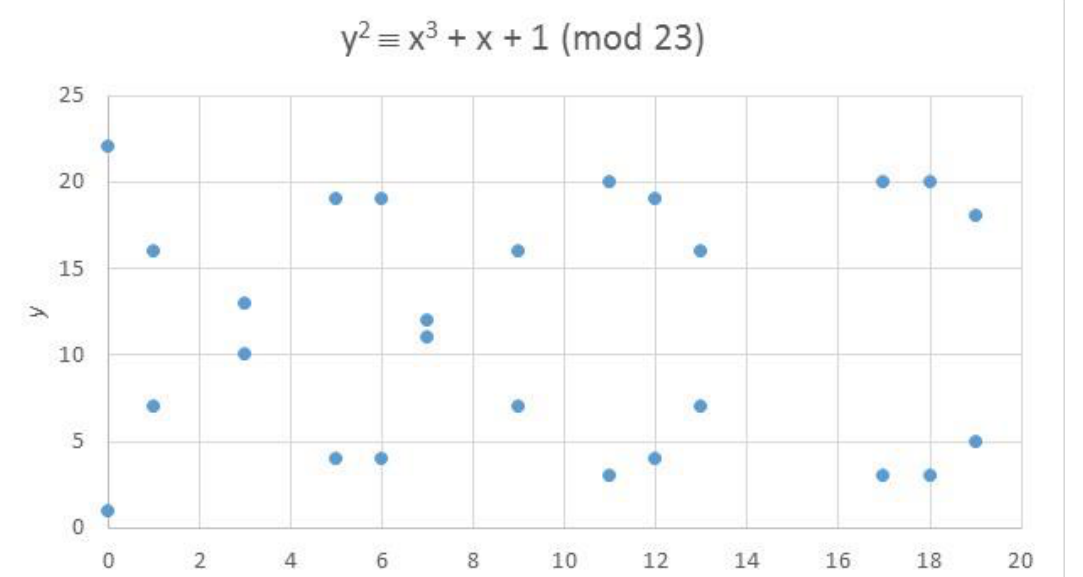
\includegraphics[width=118.44mm,height=158.89mm]{images/llm/page_029_img_01.png}%
\end{textblock*}

\newpage

% --- unit llm 30 ---
% === Halaman 30 (llm) ===

\section*{Penjumlahan Dua Titik di dalam EC pada GF(p)}

Misalkan $P(x_p, y_p)$ dan $Q(x_q, y_q)$. \\
Penjumlahan: $P + Q = R$

\subsection*{Koordinat Titik R:}
\[
\begin{aligned}
x_r &= m^2 - x_p - x_q \pmod{p} \\
y_r &= m(x_p - x_r) - y_p \pmod{p}
\end{aligned}
\]

$m$ adalah gradien:
\[
 m = \frac{y_p - y_q}{x_p - x_q} \pmod{p}
\]

\newpage

% --- unit llm 31 ---
% === Halaman 31 (llm) ===

\textbf{Pengurangan Dua Titik di dalam EC pada GF(p)}\ \\
Misalkan $P(x_p, y_p)$ dan $Q(x_q, y_q)$. \\
Pengurangan: $P - Q = P + (-Q)$, yang dalam hal ini $-Q(x_q, -y_q \pmod{p})$.

\newpage

% --- unit llm 32 ---
% === Halaman 32 (llm) ===

\section*{Penggandaan Titik di dalam EC pada GF(p)}

Misalkan $P(x_p, y_p)$ yang dalam hal ini $y_p \neq 0$.
Penggandaan titik: $2P = R$

Koordinat Titik R:
\begin{align*}
x_r &\equiv m^2 - 2x_p \pmod{p} \\
y_r &\equiv m(x_p - x_r) - y_p \pmod{p}
\end{align*}

Yang dalam hal ini,
\[ m \equiv \frac{3x_p^2 + a}{2y_p} \pmod{p} \]

Jika $y_p = 0$ maka $m$ tidak terdefinisi sehingga $2P = O$

\newpage

% --- unit llm 33 ---
% === Halaman 33 (llm) ===

\begin{itemize}
    \item \textbf{Contoh:} Misalkan $P(2, 4)$ dan $Q(5, 9)$ adalah dua buah titik pada kurva eliptik $y^2 \equiv x^3 + x + 6 \pmod{11}$. Tentukan $P + Q$ dan $2P$.
\end{itemize}

\textbf{Jawab:}\
(a) $\color{red}{P + Q = R}$
\[
\begin{aligned}
\text{m} & \equiv (9 - 4)/(5 - 2) \pmod{11} = 5/3 \pmod{11} = 5 \cdot 3^{-1} \pmod{11} \\
& = 5 \cdot 4 \pmod{11} \equiv 9 \pmod{11}
\end{aligned}
\]
$P + Q = R$, koordinat Titik R:
\[
\begin{aligned}
x_r & \equiv \text{m}^2 - x_p - x_q \pmod{11} \equiv 81 - 2 - 5 \pmod{11} \equiv 8 \pmod{11} \\
y_r & \equiv \text{m}(x_p - x_r) - y_p \pmod{11} \equiv 9(2 - 8) - 4 \pmod{11} \equiv -58 \pmod{11} \\
& \equiv 8 \pmod{11}
\end{aligned}
\]

Jadi, $R(8, 8)$

\newpage

% --- unit llm 34 ---
% === Halaman 34 (llm) ===

(b) $2P = R$

\[ m \equiv \frac{3x_p^2 + a}{2y_p} \pmod{p} \]

\begin{align*}
 m &= (3(2)^2 + 1)/8 \pmod{11} \equiv 13/8 \pmod{11} \\
 &\equiv 13 \cdot 8^{-1} \pmod{11} \\
 &\equiv 13 \cdot 7 \pmod{11} \\
 &\equiv 78 \pmod{11} \equiv 3 \pmod{11} 
\end{align*}

Koordinat R:

\begin{align*}
 x_r &\equiv m^2 - 2x_p \pmod{p} \equiv 3^2 - 2 \cdot 2 \pmod{11} \equiv 5 \pmod{11} \\
 y_r &\equiv m(x_p - x_r) - y_p \pmod{p} \equiv 3(2 - 5) - 4 \pmod{11} \\
 &\equiv -13 \pmod{11} \equiv 9 \pmod{11} 
\end{align*}

Jadi, $R(5, 9)$

\newpage

% --- unit llm 35 ---
% === Halaman 35 (llm) ===

\vspace{210.87mm}

Demo kallkulator ECC online: \url{https://andrea.corbellini.name/ecc/interactive/reals-add.html}

\vspace{10mm}

Point addition over the elliptic curve $y^2 = x^3 + 1x + 6$ in $\mathbb{F}_{11}$. The curve has 13 points (including the point at infinity).

% deskripsi: Screenshot kalkulator interaktif Elliptic Curve point addition (Fp) yang menampilkan grafik koordinat, input parameter kurva (a=1, b=6), field p=11, serta koordinat titik P, Q, dan hasil penjumlahan R=P+Q.
% bbox normalisasi: [0.0300, 0.1400, 0.9600, 0.8500]
\begin{textblock*}{195.30mm}(6.30mm,41.58mm)
\noindent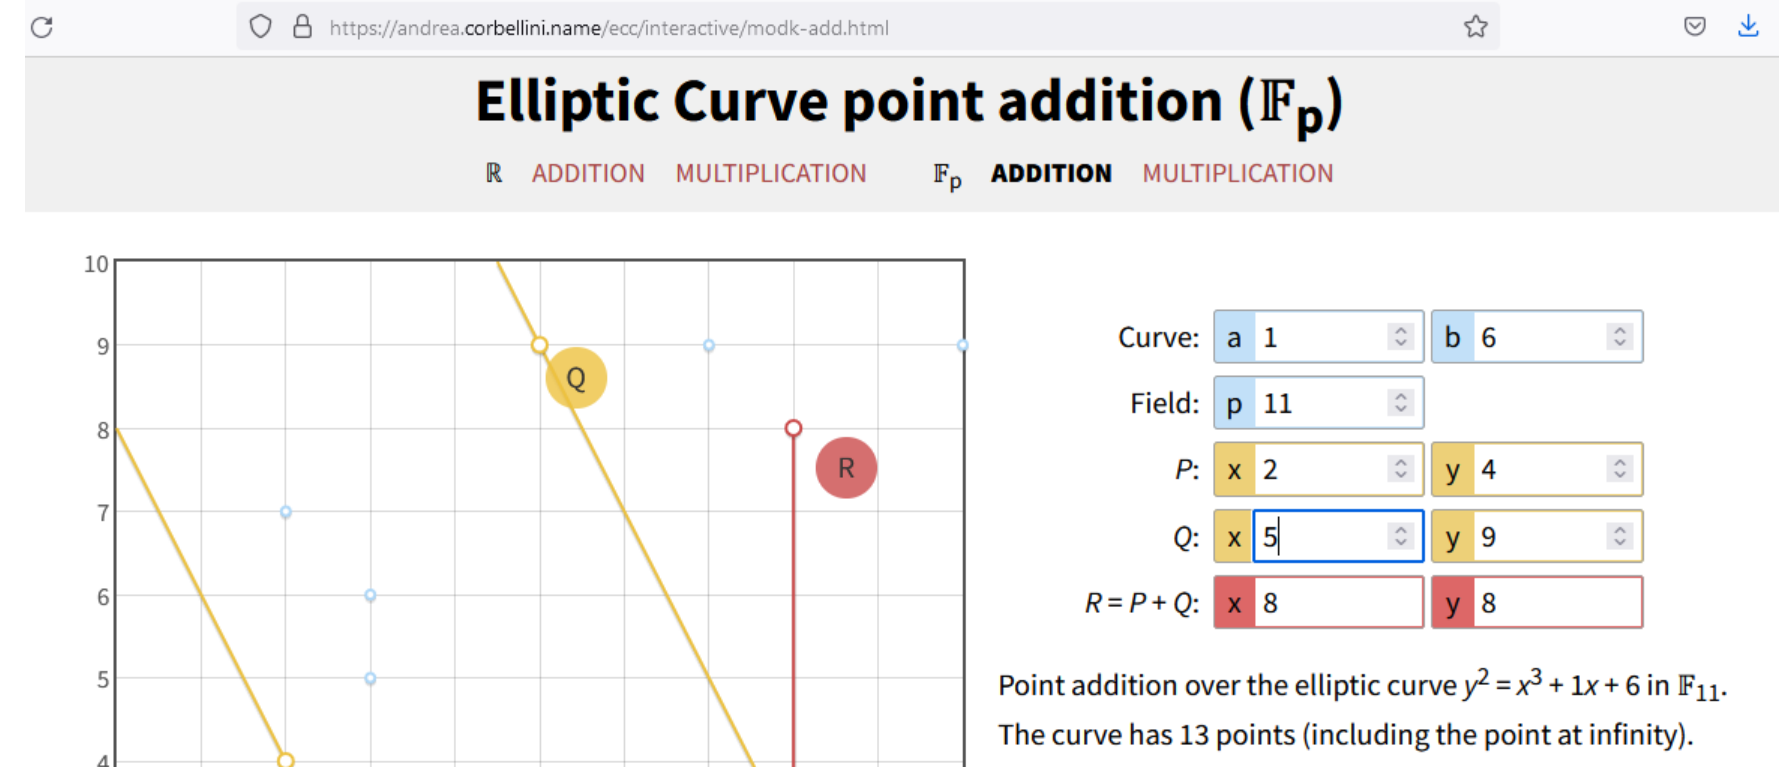
\includegraphics[width=195.30mm,height=210.87mm]{images/llm/page_035_img_01.png}%
\end{textblock*}

\newpage

% --- unit llm 36 ---
% === Halaman 36 (llm) ===

\begin{itemize}
  \item Nilai $kP$ untuk $k = 2, 3, \dots$ diperlihatkan pada tabel:
\end{itemize}

\vspace{10mm}

Jika diketahui $P$, maka kita bisa menghitung
\[ Q = kP \]

Jika persoalannya dibalik sbb:
\textcolor{red}{Diberikan $P$ dan $Q$, maka sangat sukar menghitung $k$ sedemikian sehingga $Q = kP$}

\begin{center}
  $\Downarrow$ \\
  \textbf{ECDLP}
\end{center}

% deskripsi: Tabel yang menunjukkan nilai k dan hasil kP untuk nilai k dari 1 sampai 13
% bbox normalisasi: [0.2050, 0.1710, 0.3420, 0.9170]
\begin{textblock*}{28.77mm}(43.05mm,50.79mm)
\noindent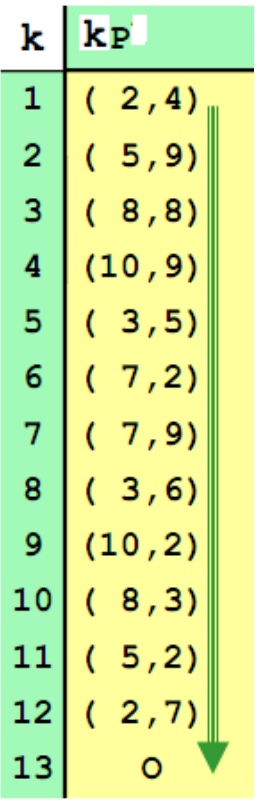
\includegraphics[width=28.77mm,height=221.56mm]{images/llm/page_036_img_01.png}%
\end{textblock*}

\newpage

% --- unit llm 37 ---
% === Halaman 37 (llm) ===

\section*{Elliptic Curve Cryptography (ECC) $\ast$)}

\begin{itemize}
    \item ECC adalah sistem kriptografi kunci-publik, sejenis dengan RSA, Rabin, ElGamal, D-H, dll.
    \item Setiap pengguna memiliki \textbf{kunci publik dan kunci privat}
    \begin{itemize}
        \item Kunci publik untuk enkripsi atau untuk verifikasi tanda tangan digital
        \item Kunci privat untuk dekripsi atau untuk menghasilkan tanda tangan digital
    \end{itemize}
    \item Kurva eliptik digunakan sebagai perluasan sistem kriptografi kunci-publik yang lain:
    \begin{enumerate}
        \item Elliptic Curve Elgamal (ECEG)
        \item Elliptic Curve Digital Signature (ECDSA)
        \item Elliptic Curve Diffie-Hellman (ECDH)
    \end{enumerate}
\end{itemize}

\vspace{10mm}

\textcolor{red}{\ast}) Sumber bahan: \textcolor{red}{Debdeep Mukhopadhyay, \textit{Elliptic Curve Cryptography}, Dept of Computer Sc and Engg IIT Madras}

\newpage

% --- unit llm 38 ---
% === Halaman 38 (llm) ===

\section*{Penggunaan Kurva Eliptik di dalam Kriptografi}

\begin{itemize}
    \item Bagian inti dari sistem kriptografi kunci-publik yang melibatkan kurva eliptik adalah \textbf{grup eliptik} (himpunan titik-titik pada kurva eliptik dan sebuah operasi biner $+$).
    \item Operasi matematika yang mendasari:
    \begin{itemize}
        \item Jika RSA mempunyai operasi perpangkatan sebagai operasi matematika yang mendasarinya, maka
        \item ECC memiliki operasi perkalian titik (kP)
    \end{itemize}
\end{itemize}

\vspace{20mm}

\begin{flushright}
\small{*) Sumber bahan: \textcolor{red}{Debdeep Mukhopadhyay, \textcolor{red}{Elliptic Curve Cryptography}, \textcolor{red}{Dept of Computer Sc and Engg IIT Madras}}
\end{flushright}

\newpage

% --- unit llm 39 ---
% === Halaman 39 (llm) ===

\begin{itemize}
    \item Dua pihak yang berkomunikasi menyepakati parameter data sebagai berikut:
    \begin{enumerate}
        \item Persamaan kurva eliptik \[ y^2 \equiv x^3 + ax + b \pmod{p} \]
        \begin{itemize}
            \item Nilai a dan b
            \item Bilangan prima p
        \end{itemize}
        \item Grup eliptik yang dihitung dari persamaan kurva eliptik
        \item Titik basis (\textit{base point}) B $(x_{\text{B}}, y_{\text{B}})$, dipilih dari grup eliptik untuk operasi kriptografi.
    \end{enumerate}
\end{itemize}

\begin{itemize}
    \item Setiap pengguna membangkitkan pasangan kunci publik dan kunci privat
    \begin{itemize}
        \item Kunci privat = integer x, dipilih dari selang $[1, p - 1]$
        \item Kunci publik = titik Q, adalah hasil kali antara x dan titik basis B: $\text{Q} = \text{x} \cdot \text{B}$
    \end{itemize}
\end{itemize}

\vfill
\raggedleft
\textcolor{red}{\small *) Sumber bahan: \textbf{Debdeep Mukhopadhyay}, \textit{Elliptic Curve Cryptography}, \\ Dept of Computer Sc and Engg IIT Madras}

\newpage

% --- unit llm 40 ---
% === Halaman 40 (llm) ===

\section*{Elliptic Curve Diffie-Hellman (ECDH)}

\vspace{172.26mm}

Ingatlah kembali diagram pertukaran kunci Diffie-Hellman:

\vspace{60mm}

% deskripsi: Diagram pertukaran kunci Diffie-Hellman yang menunjukkan langkah-langkah komputasi antara Alice dan Bob, termasuk pembangkitan angka rahasia a dan b, perhitungan nilai publik A dan B, serta penghitungan kunci bersama K.
% bbox normalisasi: [0.2200, 0.3400, 0.6700, 0.9200]
\begin{textblock*}{94.50mm}(46.20mm,100.98mm)
\noindent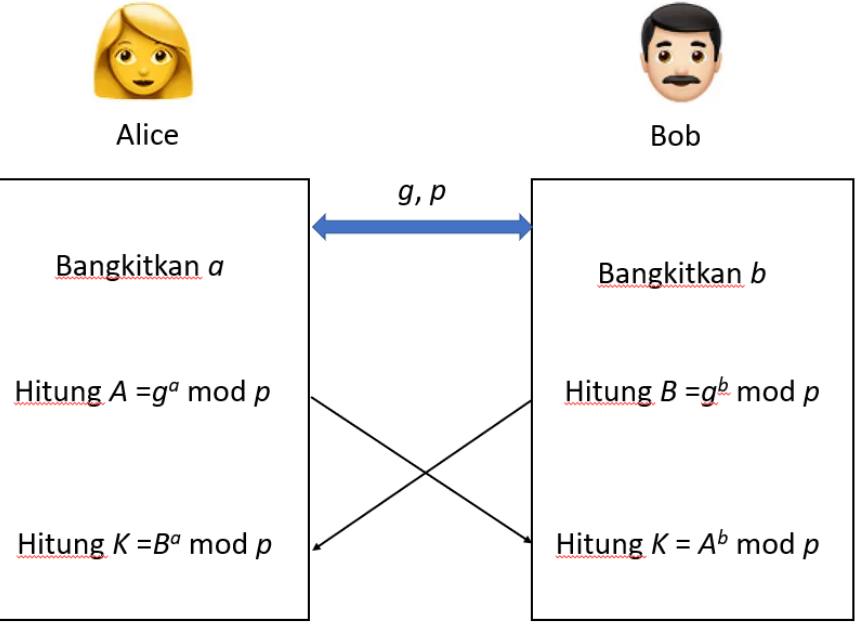
\includegraphics[width=94.50mm,height=172.26mm]{images/llm/page_040_img_01.png}%
\end{textblock*}

\newpage

% --- unit llm 41 ---
% === Halaman 41 (llm) ===

\section*{Elliptic Curve Diffie-Hellman (ECDH)}

\begin{itemize}
    \item \textbf{Public:} Kurva eliptik dan titik $B(x,y)$ pada kurva
    \item \textbf{Secret:} Integer milik Alice, $a$, dan integer milik Bob, $b$
\end{itemize}

\vspace{40mm}

\begin{itemize}
    \item Alice menghitung $K = a \cdot (b.B)$
    \item Bob menghitung $K = b \cdot (a.B)$
    \item Hasil perhitungan akan sama karena $ab = ba$
\end{itemize}

\vspace{5mm}

\textcolor{red}{(*) Sumber bahan: \textcolor{red}{Debdeep Mukhopadhyay}, \textcolor{red}{Elliptic Curve Cryptography}, \textcolor{red}{Dept of Computer Sc and Engg IIT Madras}}

% deskripsi: Diagram pertukaran kunci ECDH antara Alice dan Bob yang menunjukkan pengiriman nilai publik a.B dan b.B
% bbox normalisasi: [0.1800, 0.3400, 0.7900, 0.6300]
\begin{textblock*}{128.10mm}(37.80mm,100.98mm)
\noindent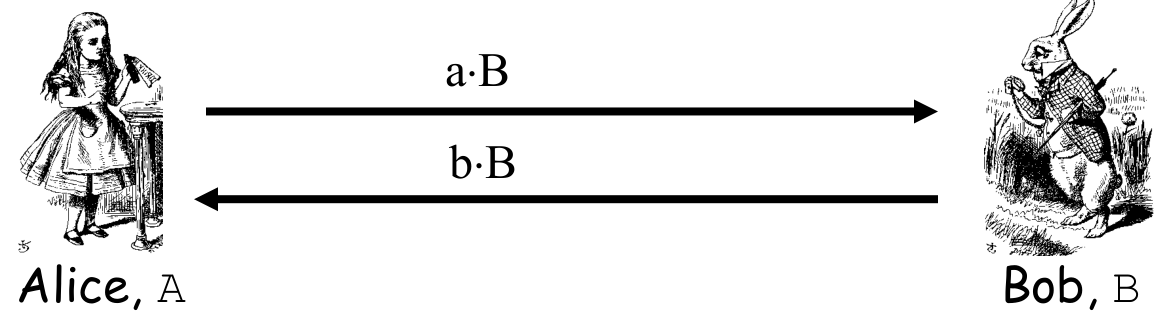
\includegraphics[width=128.10mm,height=86.13mm]{images/llm/page_041_img_01.png}%
\end{textblock*}

\newpage

% --- unit llm 42 ---
% === Halaman 42 (llm) ===

\section*{Algoritma Elliptic Curve Diffie-Hellman (ECDH)}

\begin{itemize}
    \item Alice dan Bob ingin berbagi sebuah kunci rahasia $K$ yang sama.
    \begin{itemize}
        \item Alice dan Bob menyepakati kurva eliptik $y^2 = x^3 + ax + b \pmod{p}$ dan titik $B$ pada kurva $B$
        \item Alice dan Bob menghitung kunci publik dan kunci privat masing-masing.
        \begin{itemize}
            \item Alice
            \begin{itemize}
                \item Kunci privat $= a$
                \item Kunci publik $= P_A = a \cdot B$
            \end{itemize}
            \item Bob
            \begin{itemize}
                \item Kunci privat $= b$
                \item Kunci publik $= P_B = b \cdot B$
            \end{itemize}
        \end{itemize}
    \end{itemize}
    \item Alice dan Bob saling mengirim kunci publik masing-masing.
    \item Keduanya melakukan perkalian kunci privatnya dengan kunci publik mitranya untuk mendapatkan kunci rahasia yang mereka bagi
    \begin{itemize}
        \item Alice $\rightarrow K_{AB} = a \cdot P_B = a \cdot (b \cdot B)$
        \item Bob $\rightarrow K_{AB} = b \cdot P_A = b \cdot (a \cdot B)$
        \item Kunci rahasia $= K_{AB} = abB$
    \end{itemize}
\end{itemize}

\vfill
\raggedleft
\small *) Sumber bahan: \textbf{Debdeep Mukhopadhyay}, \textit{Elliptic Curve Cryptography}, \\ Dept of Computer Sc and Engg IIT Madras

\newpage

% --- unit llm 43 ---
% === Halaman 43 (llm) ===

\textbf{Contoh *):} Misalkan kurva eliptik yang dipilih adalah $y^2 = x^3 + 2x + 1 \pmod 5$. Himpunan titik-titik pada kurva eliptik adalah $\{\{(0, 1), (1, 3), (3, 3), (3, 2), (1, 2), (0, 4)\}$. Alice dan Bob menyepakati titik $B(0, 1)$ sebagai basis.

\begin{enumerate}
    \item Alice memilih $a = 2$, lalu menghitung kunci publiknya:
    \[ P_A = a \cdot B = 2B = B + B = (1, 3) \quad \rightarrow \text{ misalkan titik Q} \]
    \item Bob memilih $b = 3$, lalu menghitung kunci publiknya:
    \[ P_B = b \cdot B = 3B = B + B + B = 2B + B = (3, 3) \quad \rightarrow \text{ misalkan titik R} \]
    \item Alice mengirimkan $P_A$ kepada Bob, Bob mengirimkan $P_B$ kepada Alice.
    \item Alice menghitung kunci rahasia sbb:
    \[ K_A = a \cdot P_B = 2R = R + R = (0, 4) \]
    \item Bob menghitung kunci rahasia sbb:
    \[ K_B = b \cdot P_A = 3Q = Q + Q + Q = (0, 4) \]
\end{enumerate}

Jadi, sekarang Alice dan Bob sudah berbagi kunci rahasia yang sama, yaitu $(0, 4)$

\vspace{10mm}
\textcolor{red}{* Sumber bahan: Nana Juhana, Implementasi Elliptic Curve Cryptography (ECC) pada proses Pertukaran Kunci Diffie-Hellman dan Skema Enkripsi El Gamal}

\newpage

% --- unit llm 44 ---
% === Halaman 44 (llm) ===

\section*{Elliptic Curve Elgamal (ECEG)}

\begin{itemize}
    \item \textit{Elliptic Curve Elgamal}: sistem kriptografi kurva eliptik yang diadopsi dari algoritma El Gamal.
    \item Misalkan \textcolor{red}{Alice} ingin mengirim \textcolor{red}{Bob} pesan M yang dienkripsi.
    \begin{itemize}
        \item Baik Alice dan Bob menyepakati kurva elelitik dan titik basis B.
        \item Alice dan Bob membuat kunci privat/kunci publik.
        \begin{itemize}
            \item Alice
            \begin{itemize}
                \item Kunci privat = a
                \item Kunci publik = $P_A = a \cdot B$
            \end{itemize}
            \item Bob
            \begin{itemize}
                \item Kunci privat = b
                \item Kunci publik = $P_B = b \cdot B$
            \end{itemize}
        \end{itemize}
    \end{itemize}
    \item Alice mengambil plainteks, M, lalu mengkodekannya menjadi sebuah titik, $P_M$, pada kurva eliptik
\end{itemize}

\vspace{5mm}

\textcolor{red}{*) Sumber bahan: Debdeep Mukhopadhyay, Elliptic Curve Cryptography , Dept of Computer Sc and Engg IIT Madras}

\newpage

% --- unit llm 45 ---
% === Halaman 45 (llm) ===

\begin{itemize}
    \item Alice memilih bilangan acak $k$ yang harus terletak di dalam selang $[1, p-1]$
    \item Cipherteks dari $P_M$ adalah pasangan titik
    \begin{itemize}
        \item $P_C = [ ( kB), (P_M + kP_B) ]$
    \end{itemize}
    \item Untuk mendekripsi, Bob mula-mula menghitung hasil kali titik pertama dari $P_C$ (yaitu $kB$) dengan kunci privatnya, $b$
    \begin{itemize}
        \item $b \cdot (kB)$
    \end{itemize}
    \item Bob kemudian mengurangkan titik kedua dari $P_C$ dengan hasil kali di atas
    \begin{itemize}
        \item $(P_M + kP_B) - [b \cdot (kB)] = P_M + k \cdot (bB) - b \cdot (kB) = P_M$
    \end{itemize}
    \item Bob kemudian men-decode $P_M$ untuk memperoleh pesan M
\end{itemize}

\vspace{10mm}

\textcolor{red}{*) Sumber bahan: Debdeep Mukhopadhyay, Elliptic Curve Cryptography , Dept of Computer Sc and Engg IIT Madras}

\newpage

% --- unit llm 46 ---
% === Halaman 46 (llm) ===

\section*{Perbandingan Elgamal dengan Elliptic Curve Elgamal}

\begin{itemize}
    \item Cipherteks pada EC-Elgamal adalah pasangan titik
    \begin{itemize}
        \item $P_C = ( (kB), (P_M + kP_B) )$ \quad (ket: $P_b = \text{kunci publik Bob}$)
    \end{itemize}
    
    \item $\color{red}{\text{Cipherteks pada Elgamal juga pasangan nilai:}}$
    \begin{itemize}
        \item $\color{red}{C = (a, b) = (g^k \pmod p, my_B^k \pmod p)$ \quad (ket: $y_b = \text{kunci publik Bob}$)}
    \end{itemize}
\end{itemize}

\hrulefill

\begin{itemize}
    \item Pada EC\_Elgamal, Bob mengurangkan titik kedua dari $P_C$ dengan hasil kali $b \cdot (kB)$
    \begin{itemize}
        \item $(P_M + kP_B) - [b(kB)] = P_M + k(bB) - b(kB) = P_M$
    \end{itemize}
    
    \item $\color{red}{\text{Pada El Gamal, Bob membagi nilai kedua dengan nilai pertama yang dipangkatkan}}$
    \color{red}{\text{dengan kunci privat Bob}}
    \begin{itemize}
        \item $\color{red}{my_B^k / (g^k)^b = mg^{k*b} / g^{k*b} = m}$
    \end{itemize}
\end{itemize}

\vspace{10mm}

\begin{flushright}
\small $\text{*)} \text{Sumber bahan: } \text{\color{blue}{Debdeep Mukhopadhyay, Elliptic Curve Cryptography,}}$ \\
\small $\text{\color{blue}{Dept of Computer Sc and Engg IIT Madras}}$
\end{flushright}

\newpage

% --- unit llm 47 ---
% === Halaman 47 (llm) ===

\section*{Encoding Pesan menjadi Titik di dalam Kurva}

\begin{itemize}
    \item Pesan yang akan dienkripsi dengan ECC harus dikonversi (\textit{encoding}) menjadi titik di dalam kurva eliptik.
    \item Metode yang sederhana adalah memetakan setiap karakter ASCII dengan setiap titik pada kurva eliptik.
    \item Untuk 256 karakter ASCII, maka dibutuhkan kurva eliptik yang berisi minimal 256 titik.
    \item Misalkan pesan $M = \text{'ENCRYPT'}$, yang dalam nilai ASCII adalah '69', '78', '67', '82', '89', '80', '84'. Setiap nilai ini dipetakan ke sebuah titik pada kurva eliptik.
    \item Namun metode ini kurang aman.
\end{itemize}

\newpage

% --- unit llm 48 ---
% === Halaman 48 (llm) ===

\begin{itemize}
    \item Metode kedua adalah dengan metode Kolbitz. Langkah-langkahnya adalah sebagai berikut:
    \begin{enumerate}
        \item Pilih sebuah kurva eliptik $y^2 \equiv x^3 + ax + b \pmod{p}$ yang mengandung $N$ buah titik.
        \item Misalkan karakter-karakter penyusun pesan adalah angka $0, 1, 2, \dots, 9$ dan huruf $A, B, C, \dots, Z$ yang dikodekan menjadi $10, 11, \dots, 35$.
        \item Kodekan setiap karakter di dalam pesan menjadi nilai $m$ di antara $0$ dan $35$.
        \item Pilih sebuah bilangan bulat $k$ sebagai parameter basis (disepakati kedua pihak).
        \item Untuk setiap nilai $mk$, nyatakan $x = mk + 1$, sulihkan $x$ ke dalam $y^2 \equiv x^3 + ax + b \pmod{p}$ lalu tentukan nilai $y$ yang memenuhi.
        \item Jika tidak ada nilai $y$ yang memenuhi, coba untuk $x = mk + 2, x = mk + 3$, dst, sampai $y^2 \equiv x^3 + ax + b \pmod{p}$ dapat dipecahkan.
        \item Pada proses \textit{decoding}, untuk titik $(x, y)$, tentukan nilai $m$ terbesar tetapi lebih kecil dari $(x - 1)/k$. Kodekan titik $(x, y)$ menjadi symbol $m$.
    \end{enumerate}
\end{itemize}

\newpage

% --- unit llm 49 ---
% === Halaman 49 (llm) ===

\textbf{Contoh:} Misalkan $y^2 \equiv x^3 - x + 188 \pmod{751}$. Kurva eliptik ini memiliki $N = 727$ buah titik.

\begin{itemize}
    \item Misalkan karakter yang akan dikodekan adalah huruf 'B', yang dikodekan menjadi nilai 11.
    \item Pilih $k = 20$, maka $x = mk + 1 = (11)(20) + 1 = 221$. Sulihkan $x = 221$ ke dalam kurva eliptik $y^2 \equiv x^3 - x + 188 \pmod{751} \equiv 456 \pmod{751}$. Tidak ada nilai $y$ yang memenuhi.
    \item Coba untuk $x = mk + 2 = (11)(20) + 2 = 222$. Sulihkan $x = 222$ ke dalam kurva eliptik $y^2 \equiv x^3 - x + 188 \pmod{751}$. Juga tidak ada nilai $y$ yang memenuhi.
    \item Coba untuk $x = mk + 3 = (11)(20) + 3 = 223$. Sulihkan $x = 223$ ke dalam kurva eliptik $y^2 \equiv x^3 - x + 188 \pmod{751}$. Juga tidak ada nilai $y$ yang memenuhi.
    \item Coba untuk $x = mk + 4 = (11)(20) + 4 = 224$. Sulihkan $x = 224$ ke dalam kurva eliptik $y^2 \equiv x^3 - x + 188 \pmod{751}$. Diperoleh $y = 248$. Jadi, karakter 'B' dikodekan menjadi titik $(224, 248)$ pada kurva eliptik.
    \item Pada proses \textit{decoding}, hitung $m = \lfloor (x - 1)/k \rfloor = \lfloor (224 - 1)/20 \rfloor = \lfloor 11.15 \rfloor = 11$. Jadi pesan semula adalah huruf 'B'.
\end{itemize}

\newpage

% --- unit llm 50 ---
% === Halaman 50 (llm) ===

\section*{Keamanan ECC}

\vspace{133.65mm}

\begin{itemize}
    \item Untuk mengenkripsi kunci AES-128 dengan algoritma kriptografi kunci public, maka:
    \begin{itemize}
        \item Ukuran kunci RSA: 3072 bit
        \item Ukuran kunci ECC cuku 256 bit saja
    \end{itemize}
    \vspace{10mm}
    \item Bagaimana cara meningkatkan keamanan RSA?
    \begin{itemize}
        \item Tingkatkan ukuran kunci
        \item \textcolor{red}{Tidak Praktis?}
    \end{itemize}
    \item Dengan ECC, pertambahan ukuran kunci tidak signifikan dibandingkan RSA
\end{itemize}

\vspace{5mm}
\begin{flushright}
\small *) Sumber bahan: \textcolor{red}{Debdeep Mukhopadhyay, Elliptic Curve Cryptography}, \textcolor{red}{Dept of Computer Sc and Engg IIT Madras}
\end{flushright}

% deskripsi: Tabel pedoman NIST untuk perbandingan ukuran kunci public (ECC dan RSA) terhadap ukuran kunci AES.
% bbox normalisasi: [0.5300, 0.2800, 0.9400, 0.7300]
\begin{textblock*}{86.10mm}(111.30mm,83.16mm)
\noindent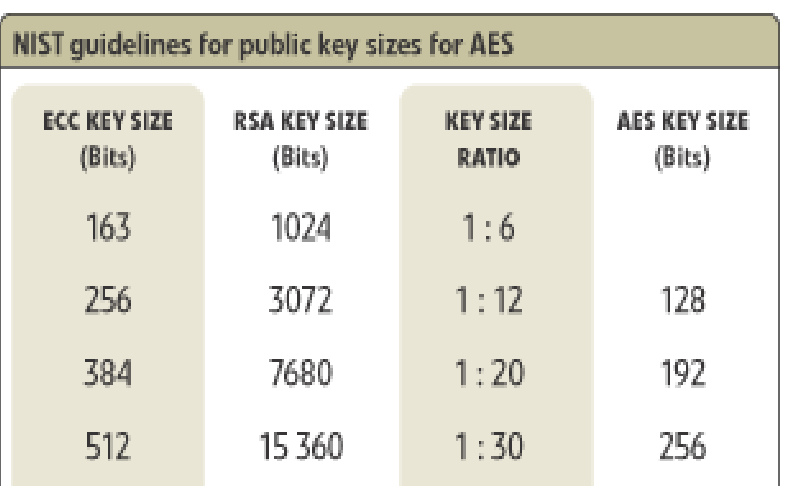
\includegraphics[width=86.10mm,height=133.65mm]{images/llm/page_050_img_01.png}%
\end{textblock*}

\newpage

% --- unit llm 51 ---
% === Halaman 51 (llm) ===

\section*{Aplikasi ECC}

\begin{itemize}
    \item Banyak piranti yang berukuran kecil dan memiliki keterbatasan memori dan kemampuan pemrosesan.
    \item Di mana kita dapat menerapkan ECC?
    \begin{itemize}
        \item Piranti komunikasi nirkabel
        \item \textit{Smart cards}
        \item Web server yang membutuhkan penanganan banyak sesi enkripsi
        \item \textcolor{red}{Sembarang aplikasi yang membutuhkan keamanan tetapi memiliki kekurangan dalam \textit{power}, \textit{storage} and kemampuan komputasi adalah potensial memerlukan ECC}
    \end{itemize}
\end{itemize}

\vspace{10mm}

\centering
\small{*) Sumber bahan: \textcolor{red}{Debdeep Mukhopadhyay}, \textcolor{red}{Elliptic Curve Cryptography}, \\ \textcolor{red}{Dept of Computer Sc and Engg IIT Madras}}

\newpage

% --- unit llm 52 ---
% === Halaman 52 (llm) ===

\section*{Keuntungan ECC}

\begin{itemize}
    \item Keuntungan yang sama dengan sistem kriptografi lain: \textit{confidentiality}, \textit{integrity}, \textit{authentication} and \textit{non-repudiation}, tetapi...
    \item Panjang kuncinya lebih pendek
    \begin{itemize}
        \item Mempercepat proses \textit{encryption}, \textit{decryption}, dan \textit{signature verification}
        \item Penghematan \textit{storage} dan \textit{bandwidth}
    \end{itemize}
\end{itemize}

\vspace{50mm}

\textcolor{red}{*) Sumber bahan: Debdeep Mukhopadhyay, Elliptic Curve Cryptography , Dept of Computer Sc and Engg IIT Madras}

\newpage

% --- unit llm 53 ---
% === Halaman 53 (llm) ===

TAMAT

\end{document}
